\documentclass{article}
\usepackage{fontenc}
\usepackage[ngerman]{babel}
\usepackage[utf8]{inputenc}
\usepackage{graphicx}
\usepackage{grffile}
\usepackage{subcaption}
\usepackage[export]{adjustbox}
\graphicspath{ {../pics/Blatt_3} }
\usepackage{alphalph}
\usepackage{amsmath}
\DeclareUnicodeCharacter{2028}{\linebreak}
\usepackage{hyperref}
\usepackage{listings}
\usepackage{color}

\definecolor{dkgreen}{rgb}{0,0.6,0}
\definecolor{gray}{rgb}{0.5,0.5,0.5}
\definecolor{mauve}{rgb}{0.58,0,0.82}

\lstset{frame=tb,
  language=Java,
  aboveskip=3mm,
  belowskip=3mm,
  showstringspaces=false,
  columns=flexible,
  basicstyle={\small\ttfamily},
  numbers=left,
  numberstyle=\tiny\color{gray},
  keywordstyle=\color{blue},
  commentstyle=\color{dkgreen},
  stringstyle=\color{mauve},
  breaklines=true,
  breakatwhitespace=true,
  tabsize=3
}
\usepackage{datetime}
\newdateformat{myformat}{\THEDAY{ten }\monthname[\THEMONTH], \THEYEAR}

\begin{document}
		\begin{titlepage}
		\centering
		{\scshape\LARGE
			Ereignisdiskrete Systeme
			\par}
		\vspace{1.5cm}
		{\huge\bfseries Praktikum Blatt 3 - Petri-Netze\par}
		\vspace{1.5cm}
		{\LARGE\itshape Jan Kristel, Alexandra Moritz\par}
		\vfill
			Aufsicht von Frau Rembold\par
			
		\vfill	
			{\large \today \par}	
		
	\end{titlepage}
	
	\tableofcontents
	\newpage
	
	\section{Petri-Netz}
		\begin{figure}[h]
			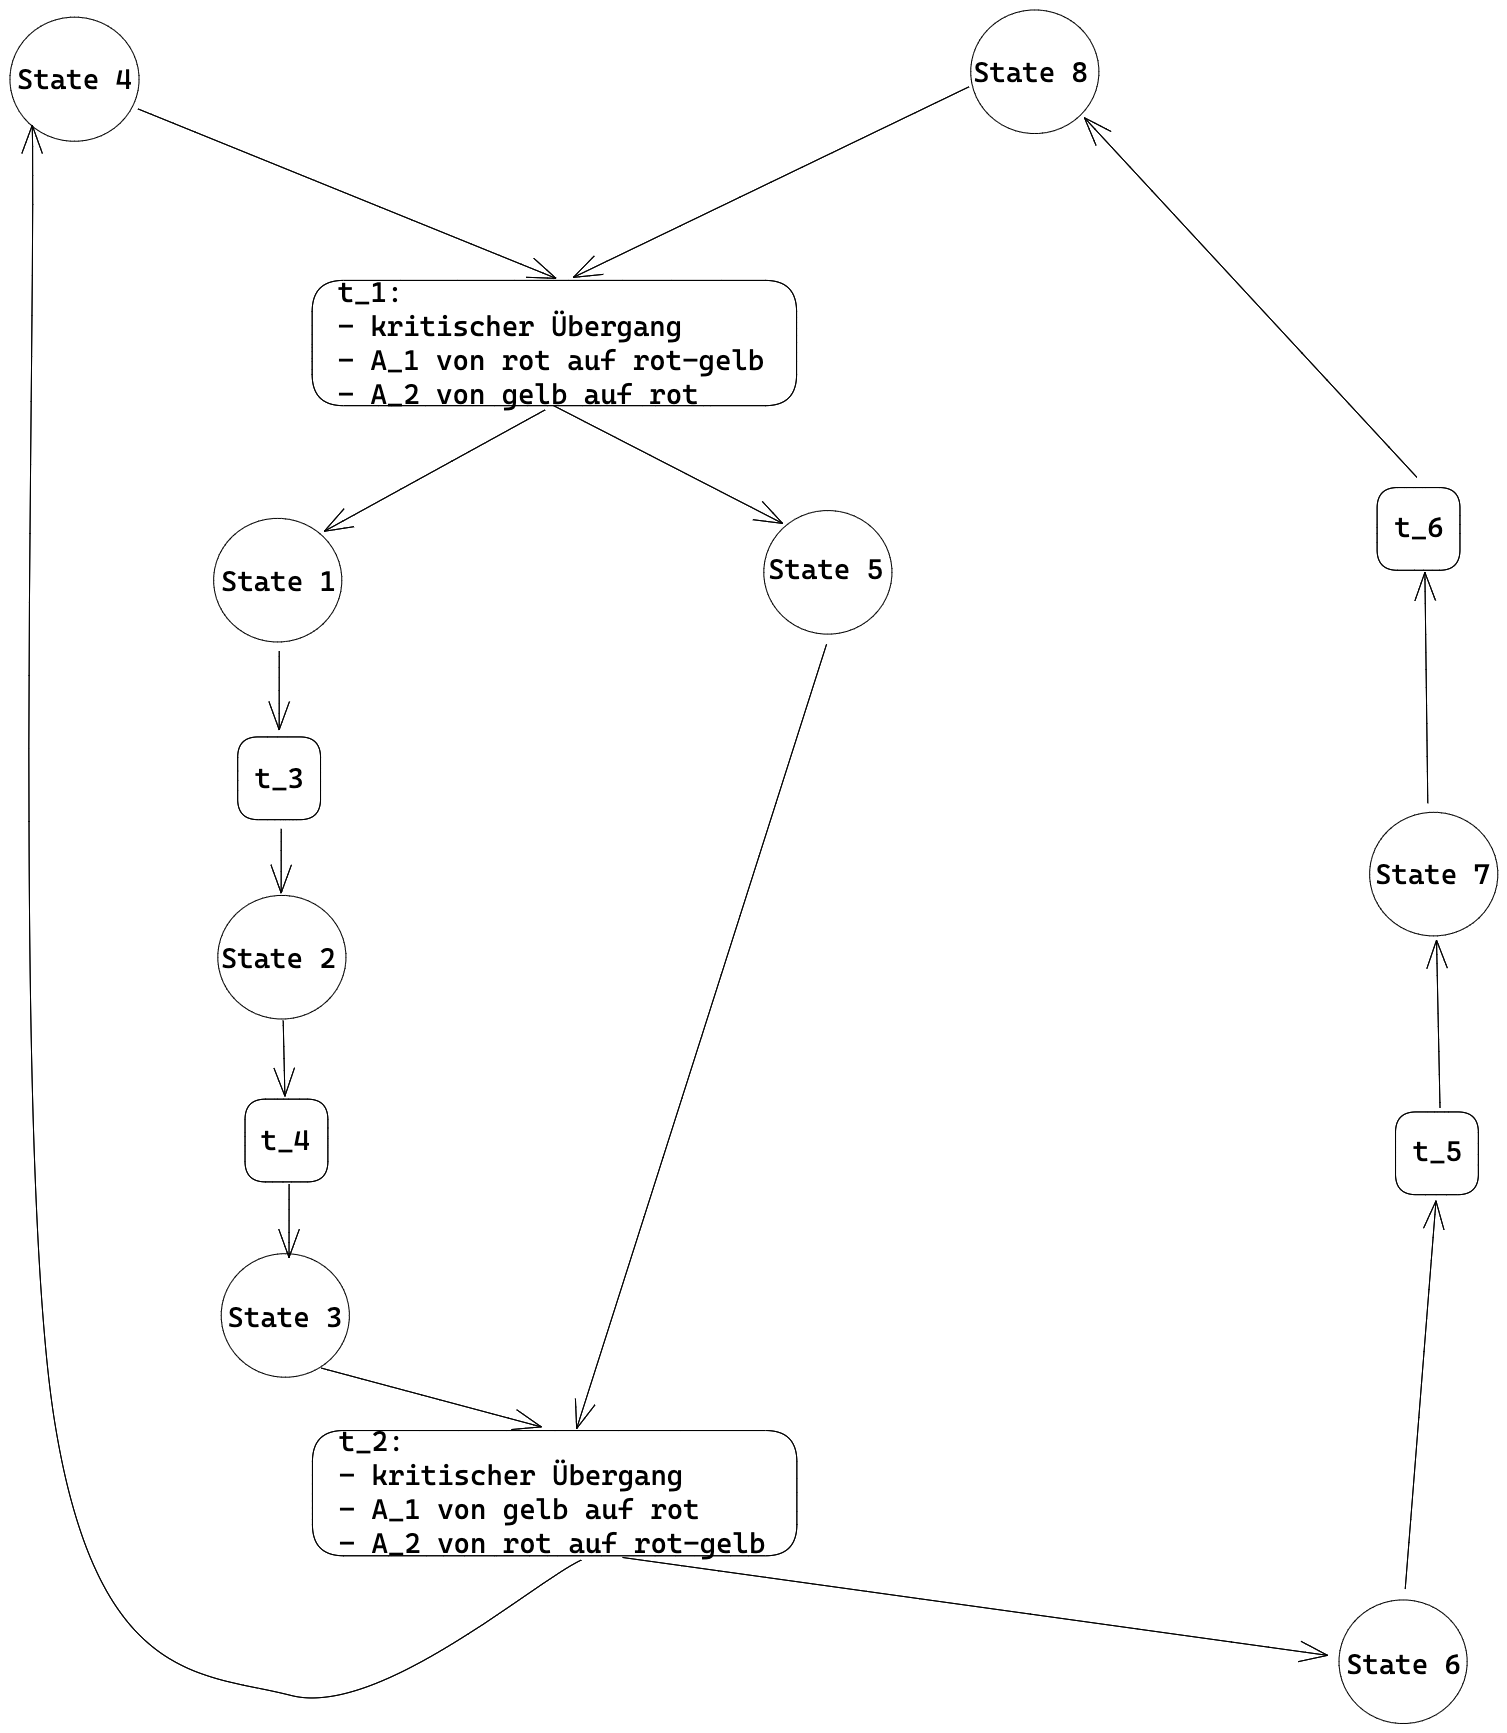
\includegraphics[scale=0.14, left ,height=0.51\paperheight ,width=\paperwidth]{Petrinetz.png}
			\caption{Petrinetz zu unserer Ampelanlage.}
			\label{fig_1: Petrinetz}
		\end{figure}
\newpage
	\section{Anfangsmarkierung}
		Als Anfangsmarkierung wurde der Zustand gewählt, den die Anlage vor de kritische Übergang $t_1$ hat, also in dem Ampel $A_1$ von \textcolor{red}{rot} auf \textcolor{red}{rot}-\textcolor{yellow}{gelb} umschält; und Ampel $A_2$ von \textcolor{yellow}{gelb} auf \textcolor{red}{rot}.
		Damit ergibt sich für die Anfangsmarkierung $m_0$ folgender Vektor:
		$$m_0 = (0\ 0\ 0\ 1\ 0\ 0\ 0\ 1)$$
	\section{Inzidenzmatrix}
		Die Inzidenzenmatrix $N$ berechnet sich als Differenz der Outputmatrix $O$ und der Inputmatrix $I$:
		$$N = O -I$$
		Die \textbf{Input}matrix sieht wie folgt aus:\\
		\begin{center}
			\begin{tabular}{| c || c c c c c c |}
				\hline
				Zustand/Übergang	 & $t_1$ & $t_2$ & $t_3$ & $t_4$ & $t_5$ & $t_6$ \\
				\hline\hline
				$S_1$ & 0 & 0 & 1 & 0 & 0 & 0\\
				$S_2$ & 0 & 0 & 0 & 1 & 0 & 0\\
				$S_3$ & 0 & 1 & 0 & 0 & 0 & 0\\
				$S_4$ & 1 & 0 & 0 & 0 & 0 & 0\\
				$S_5$ & 0 & 1 & 0 & 0 & 0 & 0\\
				$S_6$ & 0 & 0 & 0 & 0 & 1 & 0\\
				$S_7$ & 0 & 0 & 0 & 0 & 0 & 1\\
				$S_8$ & 1 & 0 & 0 & 0 & 0 & 0\\
				\hline
			\end{tabular}
		\end{center}
\vspace{5mm}
		Die \textbf{Output}matrix hat folgende Form:\\
		\begin{center}
			\begin{tabular}{| c || c c c c c c |}
				\hline
				Zustand/Übergang	 & $t_1$ & $t_2$ & $t_3$ & $t_4$ & $t_5$ & $t_6$ \\
				\hline\hline
				$S_1$ & 1 & 0 & 0 & 0 & 0 & 0\\
				$S_2$ & 0 & 0 & 1 & 0 & 0 & 0\\
				$S_3$ & 0 & 0 & 0 & 1 & 0 & 0\\
				$S_4$ & 0 & 1 & 0 & 0 & 0 & 0\\
				$S_5$ & 1 & 0 & 0 & 0 & 0 & 0\\
				$S_6$ & 0 & 1 & 0 & 0 & 0 & 0\\
				$S_7$ & 0 & 0 & 0 & 0 & 1 & 0\\
				$S_8$ & 0 & 0 & 0 & 0 & 0 & 1\\
				\hline
			\end{tabular}
		\end{center}
\newpage
		Für die \textbf{Inzidenzen}matrix ergibt sich folgenden Ergebnis:\\
		\begin{center}
			\begin{tabular}{| c || c c c c c c |}
				\hline
				Zustand/Übergang	 & $t_1$ & $t_2$ & $t_3$ & $t_4$ & $t_5$ & $t_6$ \\
				\hline\hline
				$S_1$ & 1 & 0 & $-1$ & 0 & 0 & 0\\
				$S_2$ & 0 & 0 & 1 & $-1$ & 0 & 0\\
				$S_3$ & 0 & $-1$ & 0 & 1 & 0 & 0\\
				$S_4$ & $-1$ & 1 & 0 & 0 & 0 & 0\\
				$S_5$ & 1 & $-1$ & 0 & 0 & 0 & 0\\
				$S_6$ & 0 & 1 & 0 & 0 & $-1$ & 0\\
				$S_7$ & 0 & 0 & 0 & 0 & 1 & $-1$\\
				$S_8$ & $-1$ & 0 & 0 & 0 & 0 & 1\\
				\hline
			\end{tabular}
		\end{center}
\newpage
	\section{Erreichbarkeitsgraph}
		\begin{figure}[h]
			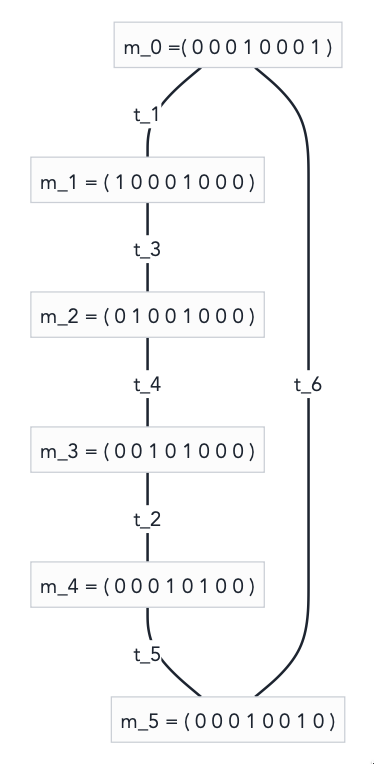
\includegraphics[scale=0.525, center]{Erreichbarkeitsgraph.png}
			\caption{Der Erreichbarketisgraph zum Petrinetz der Ampelanage}
			\label{fig_2: Erreichbarkeitsgraph}
		\end{figure}
	\section{Netzeigenschaften}
		\subsection*{Erreichbarkeit}
			Das Netz ist erreichbar, den jedes $m_i$ ist von $m_0$ aus erreichbar.
		\subsection*{Deadlock}
			Durch die Gegebenheit der Erreichbarkeit besitzt das Netz keine Deadlock.
		\subsection*{Lebendigkeit}
			Da das Netz keinen Deadlock besitzt ist es deadlockfrei, also auch lebendig.
		\subsection*{Umkehrbarkeit}
			Die Anfangsmarkierung $m_0$ kann, auch durch den zyklischen Ablauf, von jeder Markierung $m_i$ erreicht werden. D.h. es ist umkehrbar.
		\subsection*{Konfliktfreiheit}
			Das Netz der Ampelanlage ist konfliktfrei, da keine Aktivierung eines Übergangs, die Aktivierung eines anderen Übergangs verhindert indem ihm ein Token entzogen wird.
		\subsection*{Beschränktheit}
			Die Ampelanlage ist $1$-beschränkt. Kein Zustand innerhalb des Petrinetzes besitzt jemals mehr als $1$ Token.
	\section{Schaltvektor}
		Der Schaltvektor $v$ entsteht bei Muliplikation von Inputmatrix $I$ und dem Vektor selbst, wobei das Produkt $0$ ergeben muss.
		$$0 = I \cdot v$$
		Der Vektor $v$ hat dabei die gleiche Größe wie Anzahl an Übergängen im Netz. Womit dieser zunächst so aussieht:\\
		$$v =
			\begin{pmatrix}
				v_1\\
				v_2\\
				v_3\\
				v_4\\
				v_5\\
				v_6\\
				v_7\\
				v_8			
			\end{pmatrix}
		$$
\newpage
		Multipliziert mit der Inputmatrix $I$
		\begin{center}
			\begin{tabular}{| c || c c c c c c |}
				\hline
				Zustand/Übergang	 & $t_1$ & $t_2$ & $t_3$ & $t_4$ & $t_5$ & $t_6$ \\
				\hline\hline
				$S_1$ & 0 & 0 & 1 & 0 & 0 & 0\\
				$S_2$ & 0 & 0 & 0 & 1 & 0 & 0\\
				$S_3$ & 0 & 1 & 0 & 0 & 0 & 0\\
				$S_4$ & 1 & 0 & 0 & 0 & 0 & 0\\
				$S_5$ & 0 & 1 & 0 & 0 & 0 & 0\\
				$S_6$ & 0 & 0 & 0 & 0 & 1 & 0\\
				$S_7$ & 0 & 0 & 0 & 0 & 0 & 1\\
				$S_8$ & 1 & 0 & 0 & 0 & 0 & 0\\
				\hline
			\end{tabular}
		\end{center}
		erhält man folgende Zeilengleichenung:
		$$v_1 + 0 - v_3 + 0 + 0 + 0 = 0$$
		$$0 + 0 + v_3 - v_4 + 0 + 0 = 0$$
		$$0 - v_2 + 0 + v_4 + 0 + 0 = 0$$
		$$-v_1 + v_2 + 0 + 0 + 0 + 0 = 0$$
		$$v_1 + v_2 + 0 + 0 + 0 + 0 = 0$$
		$$0 + v_2 + 0 + 0 - v_5 + 0 = 0$$
		$$0 + 0 + 0 + 0 + v_5 - v_6= 0$$
		$$-v_1 + 0 + 0 + 0 + 0 + v_6= 0$$
\vspace{5mm}
		Um nun wahre Aussagen für die Gleichungen zu bekommen, reicht es eine 1 für die Variablen einzusetzen. Daraus erhält man den Schaltvektor für das Petrinetz der Ampelage in folgender Form:
		$$v = 
			\begin{pmatrix}
				1\\
				1\\
				1\\
				1\\
				1\\
				1\\
				1\\
				1			
			\end{pmatrix}
		$$
\newpage
	\section{Nachweis für den Schaltevektor und die Schaltsequenz $\sigma$}
		Den Nachweis für den Schaltvektor erhält man über die Marken $m_i$ des Erreichbarkeitsgraphen.
		Jede Marke, d.h. jeder Zustand hat einen eigenen Vektor, der diesen beschreibt.\\
		Die Schaltsequenz beschreibt dabei, welche Stellen sich Vektor \textit{schalten} um zu dem nächsten Zustand zu gelangen. Für des Petrinetz der Ampelanlage hat dieses Vorgehen folgende Form:
		\begin{itemize}
			\item $m_0$
			\begin{itemize}
				\item $m_0 = (0\ 0\ 0\ 1\ 0\ 0\ 0\ 1)$
				\item Schaltvektor $v_0 = [0\ 0\ 0\ 1\ 0\ 0\ 0\ 1]$
				\item Schaltsequenz $\sigma_0 =$ T4 T8
			\end{itemize}
			\item $m_1$
			\begin{itemize}
				\item $m_1 = (1\ 0\ 0\ 0\ 1\ 0\ 0\ 0)$
				\item $v_1 = [1\ 0\ 0\ 0\ 1\ 0\ 0\ 0]$
				\item $\sigma_1 =$ T1 T5
			\end{itemize}
			\item $m_2$
			\begin{itemize}
				\item $m_2 = (0\ 1\ 0\ 0\ 1\ 0\ 0\ 0)$
				\item $v_2 = [0\ 1\ 0\ 0\ 1\ 0\ 0\ 0]$
				\item $\sigma_2 =$ T2 T5
			\end{itemize}
			\item $m_3$
			\begin{itemize}
				\item $m_3 = (0\ 0\ 1\ 0\ 1\ 0\ 0\ 0)$
				\item $v_3 =[0\ 0\ 1\ 0\ 1\ 0\ 0\ 0]$
				\item $\sigma_3 =$ T3 T5
			\end{itemize}
			\item $m_4$
			\begin{itemize}
				\item $m_4 = (0\ 0\ 0\ 1\ 0\ 1\ 0\ 0)$
				\item $v_4 = [0\ 0\ 0\ 1\ 0\ 1\ 0\ 0]$
				\item $\sigma_4 =$ T4 T6		
			\end{itemize}
			\item $m_5$
			\begin{itemize}
				\item $m_5 = (0\ 0\ 0\ 1\ 0\ 0\ 1\ 0)$
				\item $v_5 = [0\ 0\ 0\ 1\ 0\ 0\ 1\ 0]$
				\item $\sigma_5 =$ T4 T7
			\end{itemize}
		\end{itemize}
		
\newpage
	\section{Modellierung auf academic.signavio.com}
		\begin{figure}[h]
			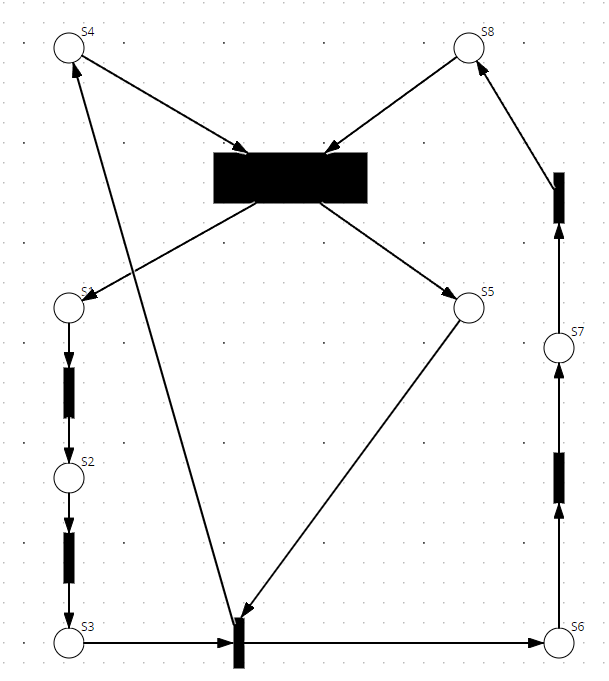
\includegraphics[scale=0.55, center]{petrinet_01_signavio.png}
			\caption{Petrinetz erstellt mit Hilfe des Tools auf academic.signavio.com/p}
			\label{fig_3: petrinet_01}
		\end{figure}
\newpage
	\section{Modellierung mit PIPE - Platform Independent Petri Net Editor v4.3.0: Petri net 1}
		\begin{figure}[h]
			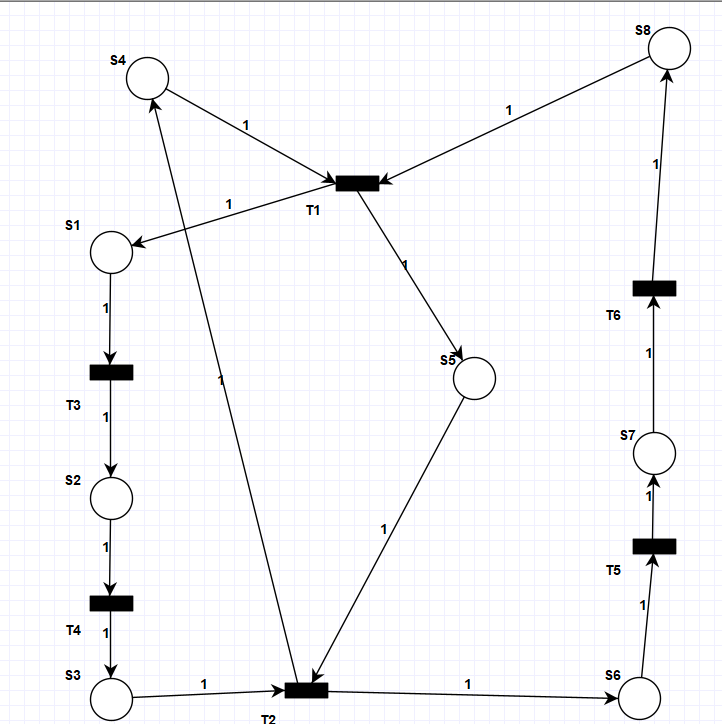
\includegraphics[scale=0.55, center]{petrinet_02_software.png}
			\caption{Ein Petrinetz zur Ampelanlage. Erstellt mir mit dem PIPE-Tool.}
			\label{fig_4: petrinet_02_PIPE}
		\end{figure}
\newpage
	\section{Vor- und Nachteile von Petri06 und PetriEdiSim}
		\subsection*{academic.signavio}
			Der große Vorteil des Tools der Webseite ist die einfache Bedienung und Bildsimulation der erstellten Petrinetze. Dem gegenüber steht eine kompliziert Registrierung, die für Nichthochschulemitglieder kostenpflichtig ist. Des weiteren lassen sich die Transitionen im Editor, anders als beschrieben, nicht drehen.
		\subsection*{PIPE}
			Die Software PIPE überzeugt durch eine noch einfache Bedienung. Es lassen sich Punkte/Transitionen beliebig drehen, verschieben und beschriften, ob im Editor oder innerhalb der Simulation.
			Der Nachteil hierbei ist, dass ein extra Programm heruntergeladen und installiert werden muss.
	
\end{document}